\begin{refsection}
\chapter[The Ag1000G phase 1 data resource]{The \textit{Anopheles gambiae} 1000 Genomes Project phase 1 nucleotide variation data resource}\label{ch:3}


%%%%%%%%%%%%%%%%%%%%%%%%%%%%%%%%%%%%%%%%%%%%%%%%%%%%%%%%%%%%%%%%%%%%%%%%%%%%%%%
%%%%%%%%%%%%%%%%%%%%%%%%%%%%%%%%%%%%%%%%%%%%%%%%%%%%%%%%%%%%%%%%%%%%%%%%%%%%%%%
%%%%%%%%%%%%%%%%%%%%%%%%%%%%%%%%%%%%%%%%%%%%%%%%%%%%%%%%%%%%%%%%%%%%%%%%%%%%%%%
\begin{abstract}


In this chapter I describe the production and curation of a data resource of nucleotide variation obtained from whole-genome sequencing of 888 individual mosquitoes wild-caught from natural populations, and a further 80 individuals from colony crosses.
%
Production of this data resource was a collaborative effort involving members of multiple research teams within the Ag1000G Consortium.
%
My contribution, described in this chapter, was to analyse the raw variant calls, define and carry out quality control and validation analyses, investigate genome accessibility and define quality filters, and produce the final analysis-ready data resource.
%
I also report analyses of these data to quantify the levels of nucleotide variation found, and to explore how genomic features such as protein-coding genes affect the genomic landscape of nucleotide variation.


\end{abstract}


%%%%%%%%%%%%%%%%%%%%%%%%%%%%%%%%%%%%%%%%%%%%%%%%%%%%%%%%%%%%%%%%%%%%%%%%%%%%%%%
%%%%%%%%%%%%%%%%%%%%%%%%%%%%%%%%%%%%%%%%%%%%%%%%%%%%%%%%%%%%%%%%%%%%%%%%%%%%%%%
%%%%%%%%%%%%%%%%%%%%%%%%%%%%%%%%%%%%%%%%%%%%%%%%%%%%%%%%%%%%%%%%%%%%%%%%%%%%%%%
\section{Introduction}\label{sec:ch3-introduction}


As described in chapter 1, the Ag1000G Project aims to use whole-genome deep Illumina sequencing to explore natural genetic variation among populations of malaria vectors within the \agam\ complex.
%
For logistical reasons the project was divided into three phases, and a total of 888 mosquito specimens sampled from natural populations were included in the first project phase.
%
A further 80 mosquito specimens comprising parents and progeny of four colony crosses were also sequenced within this project phase.
%
This chapter is primarily methodological, describing the processes and analyses developed and used to identify, genotype and validate single nucleotide polymorphisms (SNPs) among these specimens.
%
For completeness, I have included some brief methodological information regarding population sampling and whole-genome sequencing which were performed by members of the Ag1000G Consortium.
%
However, the main focus of this chapter is the work I contributed to production and validation of a high quality genome-wide resource of SNP data from sequencing of these specimens.
%
Where work was carried out by or in collaboration with other members of the Ag1000G Consortium I have indicated that within the relevant subsection.



%%%%%%%%%%%%%%%%%%%%%%%%%%%%%%%%%%%%%%%%%%%%%%%%%%%%%%%%%%%%%%%%%%%%%%%%%%%%%%%
%%%%%%%%%%%%%%%%%%%%%%%%%%%%%%%%%%%%%%%%%%%%%%%%%%%%%%%%%%%%%%%%%%%%%%%%%%%%%%%
%%%%%%%%%%%%%%%%%%%%%%%%%%%%%%%%%%%%%%%%%%%%%%%%%%%%%%%%%%%%%%%%%%%%%%%%%%%%%%%
\section{Methods}\label{sec:ch3-methods}


%%%%%%%%%%%%%%%%%%%%%%%%%%%%%%%%%%%%%%%%%%%%%%%%%%%%%%%%%%%%%%%%%%%%%%%%%%%%%%%
%%%%%%%%%%%%%%%%%%%%%%%%%%%%%%%%%%%%%%%%%%%%%%%%%%%%%%%%%%%%%%%%%%%%%%%%%%%%%%%
\subsection{Population sampling}\label{subsec:population-sampling}


\begin{figure}[t!]
\centering
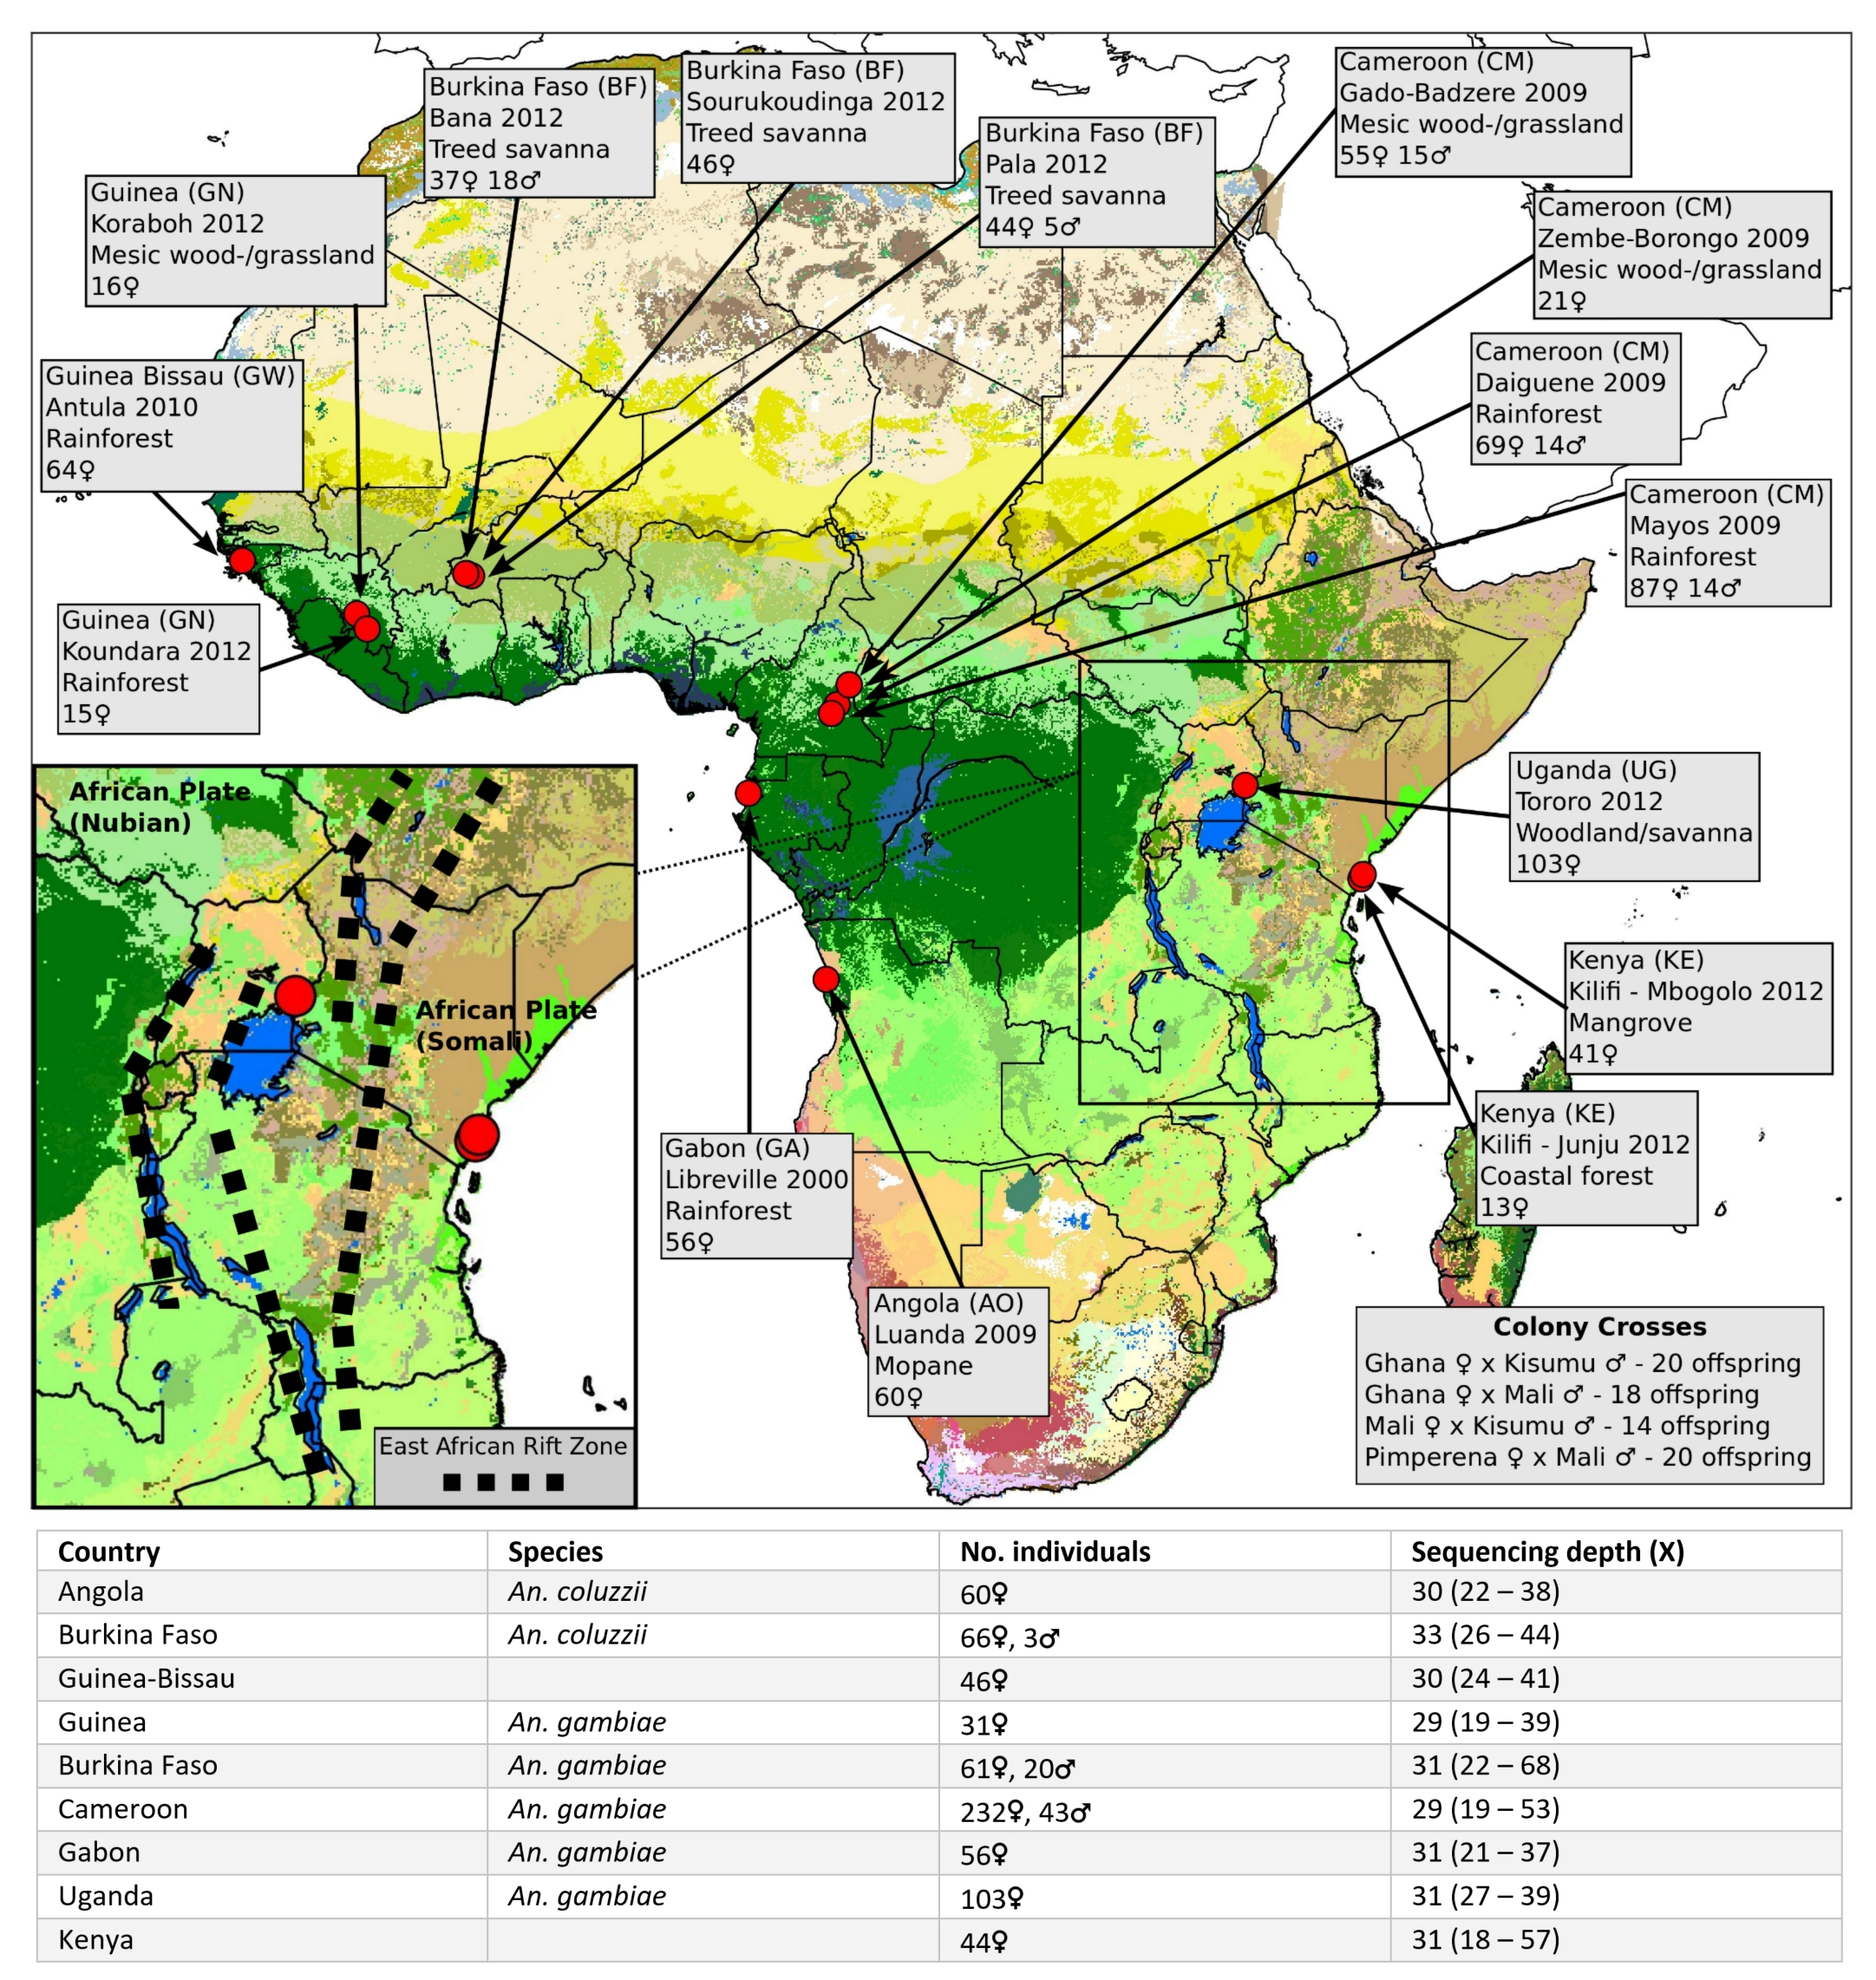
\includegraphics[width=\textwidth]{artwork/chapter3/map.jpeg}
\caption{Map of sampling locations.
%
Numbers of specimens are shown by gender.
%
Parental colonies and numbers of offspring for colony crosses are shown inset.
%
Numbers of samples are shown after removing samples that failed any of the quality control steps described in this chapter. 
%
Colours in the map denote ecosystem classes, see \textcite{Sayre2013} Fig. 9 for a complete colour legend. 
%
This figure was produced in collaboration with Chris Clarkson.}
\label{fig:ch3-map}
\end{figure}


\textit{Population sampling was performed by members of the Ag1000G Consortium. Below is a brief description of the cohort of mosquito specimens obtained for sequencing. A more detailed description is available in \textcite{Ag1000G2017}.}


%%
A total of 888 mosquito specimens collected from natural populations were included in the Ag1000G phase 1 cohort.
%
This included mosquitoes representing two major malaria vector species \agam\ and \textit{An. coluzzii}.
%
Mosquitoes were sampled from 8 countries in sub-Saharan Africa representing a broad geographical range spanning the continent: Guinea-Bissau, Guinea, Burkina Faso, Cameroon, Gabon, Angola, Uganda and Kenya (Fig.~\ref{fig:ch3-map}).
%
Mosquitoes had been collected prior to the initiation of the Ag1000G Project as part of previous field studies, and were collected at different times, with the earliest collections being in 2000 (Gabon) and the most recent in 2012 (Burkina Faso).
%
Because these mosquitoes were collected in the context of different studies, a number of different collection methods were used, including light traps, pyrethrum spray catch and larval collection.
%
In addition to the wild-caught specimens, a further 80 mosquitoes were obtained from four colony crosses, each cross comprising two parents and up to 20 progeny, where parents were drawn from established reference colonies (Fig.~\ref{fig:ch3-map} inset).
%
The main rationale for including colony crosses was to provide a mechanism for calibrating and measuring the accuracy of variant calling methods, because colony crosses allow for the analysis of genetic inheritance and Mendelian inconsistencies between parents and offspring, which can be a useful proxy of variant calling errors~\parencite{Saunders2007,Laurie2010,Pilipenko2014}.
%
DNA extraction was performed on individual mosquitoes and genomic DNA samples were shipped to the Wellcome Sanger Institute for sequencing.


%%%%%%%%%%%%%%%%%%%%%%%%%%%%%%%%%%%%%%%%%%%%%%%%%%%%%%%%%%%%%%%%%%%%%%%%%%%%%%%
%%%%%%%%%%%%%%%%%%%%%%%%%%%%%%%%%%%%%%%%%%%%%%%%%%%%%%%%%%%%%%%%%%%%%%%%%%%%%%%
\subsection{Whole-genome sequencing}\label{subsec:whole-genome-sequencing}


\textit{Whole-genome sequencing was performed by staff at the MalariaGEN Resource Center and the Wellcome Sanger Institute sample logistics, sequencing and informatics facilities. Below is a brief description of sequencing methods. A more detailed description is available in \textcite{Ag1000G2017}.}


%%
Sequencing was performed on the Illumina HiSeq 2000 platform at the Wellcome Sanger Institute.
%
Paired-end multiplex libraries were prepared using the manufacturer's protocol, with the exception that genomic DNA was fragmented using Covaris Adaptive Focused Acoustics rather than nebulization.
%
Multiplexes comprised 12 tagged individual mosquitoes and three lanes of sequencing were generated for each multiplex to even out variations in yield between sequencing runs.
%
Thus, after sequencing data were demultiplexed, data for each individual sample were available from three separate sequencing runs.
%
Cluster generation and sequencing were undertaken per the manufacturer's protocol for paired-end 100 bp sequence reads with insert size in the range 100--200 bp.
%
Target coverage was $30\times$ per individual.
%
The median depth of coverage obtained per individual was at least $29\times$ for all the sample sets contributed (Table~\ref{table:coverage}).
%

\begin{table}[t]
\begin{center}
\begin{threeparttable}

\caption{Depth of coverage.
Coverage column shows median (interquartile range) depth coverage for all samples by country and species.
%
Numbers of samples and coverage values are shown after removing samples that failed any of the quality control steps described in this chapter. 
%
Species status is uncertain for samples from Guinea-Bissau and Kenya, see Chapter 4 for further explanation.
}

\label{table:coverage}

\begin{tabular}{llll}
 \hline
 \textbf{Country} & \textbf{Species} & \textbf{No. samples} (\female, \male) & \textbf{Coverage} \\
 \hline
 Angola & \acol\ & 60, 0 & 30 (22-38) \\
 Burkina Faso & \acol\ & 66, 3 & 33 (26-44) \\
 Burkina Faso & \agam\ & 61, 20 & 31 (22-68) \\
 Cameroon & \textit{An gambiae} & 232, 43 & 29 (19-53) \\
 Gabon & \agam\ & 56, 0 & 31 (21-37) \\
 Guinea & \agam\ & 31, 0 & 29 (19-39) \\
 Uganda & \agam\ & 103, 0 & 31 (27-39) \\
 Guinea Bissau & uncertain & 46, 0 & 30 (24-41) \\
 Kenya & uncertain & 44, 0 & 31 (18-57) \\
 \hline
\end{tabular}

\end{threeparttable}
\end{center}
\end{table}


%%%%%%%%%%%%%%%%%%%%%%%%%%%%%%%%%%%%%%%%%%%%%%%%%%%%%%%%%%%%%%%%%%%%%%%%%%%%%%%
%%%%%%%%%%%%%%%%%%%%%%%%%%%%%%%%%%%%%%%%%%%%%%%%%%%%%%%%%%%%%%%%%%%%%%%%%%%%%%%
\subsection{SNP discovery and genotyping}\label{subsec:snp-discovery-and-genotyping}


\textit{SNP discovery and genotyping was performed in collaboration with the MalariaGEN Resource Center data production team. Below is a brief description of SNP calling methods. A more detailed description is available in \textcite{Ag1000G2017}.}


%%
SNP discovery and genotyping was performed following best practices defined for the Genome Analysis Toolkit (GATK) version 2~\parencite{McKenna2010,Depristo2011,VanderAuwera2013}.
%
Sequence reads from each sample were aligned to the AgamP3 reference genome~\parencite{Holt2002,Sharakhova2007} using BWA version 0.6.2~\parencite{Li2009}.
%
A BAM file for each individual was constructed by merging alignments from multiple lanes, and duplicate reads were marked using Picard version 1.96.
%
Reads were then re-aligned around putative indels found within the alignments using GATK.
%
SNP discovery and genotyping was performed using GATK \textit{UnifiedGenotyper}.
%
\textit{UnifiedGenotyper} was run within non-overlapping 10 kb chunks, and the results were combined into a single variant call format (VCF) file for each chromosome arm using the \textit{vcf-concat} command from vcftools version 0.1.10.
%
SNP discovery was performed using the 888 wild-caught samples.
%
The colony crosses samples were then genotyped at the same set of SNPs using GATK \textit{UnifiedGenotyper}.


%%%%%%%%%%%%%%%%%%%%%%%%%%%%%%%%%%%%%%%%%%%%%%%%%%%%%%%%%%%%%%%%%%%%%%%%%%%%%%%
%%%%%%%%%%%%%%%%%%%%%%%%%%%%%%%%%%%%%%%%%%%%%%%%%%%%%%%%%%%%%%%%%%%%%%%%%%%%%%%
\subsection{Sample quality control}\label{subsec:sample-quality-control}


%
A number of issues can arise in the process of sample and library preparation and high-throughput sequencing which result in data of insufficient quality to perform robust variant discovery and genotyping.
%
These issues include:
%
\begin{itemize}
%
\item \textbf{Low yield.} The number of sequence reads generated for an individual sample is not sufficient to achieve the desired depth of coverage.
%
\item \textbf{Low library complexity.} If the input DNA quantity is insufficient, the DNA amplification process can generate sufficient material for sequencing, but there may be significant bias, in the sense that some genome regions are overrepresented and others are underrepresented or not covered at all~\parencite{Head2014}.
%
\item \textbf{Cross-contamination.} During specimen handling, sample preparation and library preparation, material and thus DNA from one sample may contaminate another.
%
In this case the sequencing data generated will include a mixture of reads from the original sample and the contaminating sample.
%
\item \textbf{Metadata errors.} Errors may arise during the recording and transfer of metadata about specimens and samples between information systems.
%
This can lead to situations where the identity of one sample becomes swapped with that of another sample.
%
\item \textbf{Unexpected taxa.} In Ag1000G phase 1 only \agam\ and \acol\ mosquitoes were to be included.
%
However, not all specimens had the conventional diagnostic species assays performed prior to selection, and thus were only identified morphologically.
\end{itemize}
%
In this subsection I describe analyses performed to identify and exclude samples affected by one or more of these issues.


%%%%%%%%%%%%%%%%%%%%%%%%%%%%%%%%%%%%%%%%%%%%%%%%%%%%%%%%%%%%%%%%%%%%%%%%%%%%%%%
\subsubsection{Sequencing data quality}


\begin{figure}[t!]
\centering
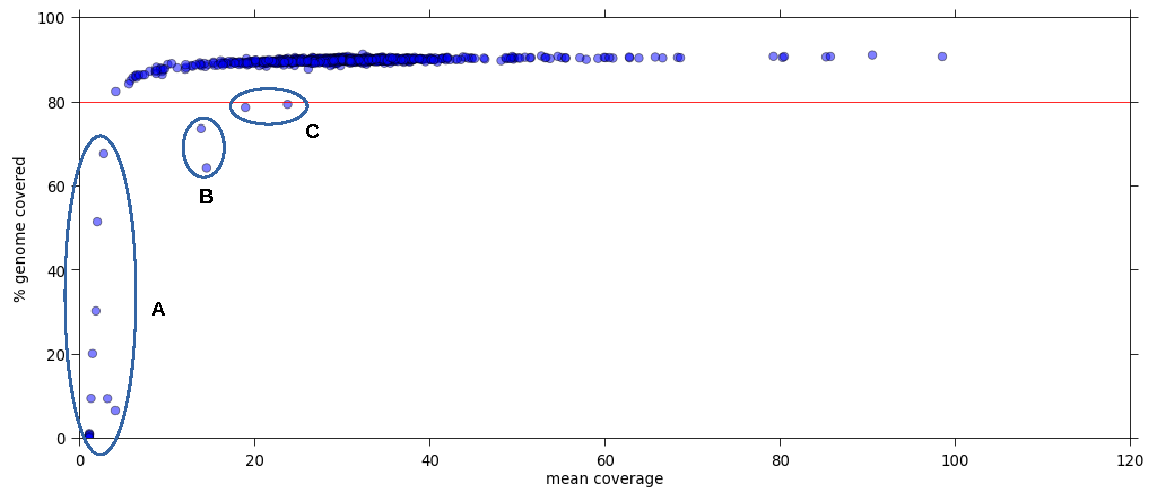
\includegraphics[width=\textwidth]{artwork/chapter3/coverage.pdf}
\caption{Sequencing data quality diagnostics.
%
Each marker represents an individual sample.
%
Mean coverage is computed as total number of sequenced bases divided by genome size.
%
Percent genome covered is percent of nucleotides in reference genome with at least one read aligned.
%
Highlighted groups A, B and C indicate different quality issues, described in the text.
}
%
\label{fig:ch3-coverage}
\end{figure}


%%
I analysed summary statistics generated from the sequence read alignments to identify samples with sequencing data quality issues such as low yield or low library complexity.
%
These statistics included the number of sequence reads, mean coverage, percentage of reads mapped to the reference genome, percentage of reads marked as duplicates, and percentage of aligned bases mismatching the reference genome.
%
I plotted various combinations of these statistics to investigate their distributions and identify outliers.
%
A particularly informative plot was to compare the mean coverage with the percentage of genome covered by at least one read (Fig.~\ref{fig:ch3-coverage}).
%
Most samples obtained greater than 80\% of the genome covered, but a set of 13 samples had both mean coverage below $7\times$ and less than 80\% of the genome covered, indicating insufficient coverage due to low sequencing yield (Fig.~\ref{fig:ch3-coverage} group A).
%
There were also four samples with high mean coverage but less than 80\% genome covered.
%
Two of these samples had a high rate of duplicate reads, and thus poor genome coverage was likely due to low library complexity (Fig.~\ref{fig:ch3-coverage} group B).
%
The remaining two samples had a higher mismatch rate, thus poor genome coverage was likely due to an unexpected taxon with higher divergence from the reference genome (Fig.~\ref{fig:ch3-coverage} group C).
%
On the basis of these analyses, the percentage of genome covered appeared to be a useful metric capturing multiple quality issues, and I excluded 17 samples with less than 80\% genome covered.
%


%%%%%%%%%%%%%%%%%%%%%%%%%%%%%%%%%%%%%%%%%%%%%%%%%%%%%%%%%%%%%%%%%%%%%%%%%%%%%%%
\subsubsection{Cross-contamination}


\begin{figure}[t!]
\centering
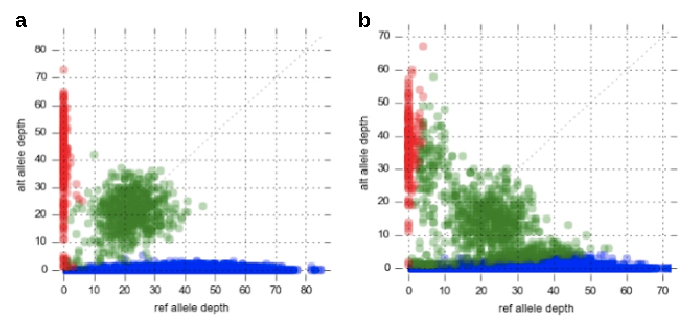
\includegraphics[width=\textwidth]{artwork/chapter3/contamination.pdf}
\caption{Cross-contamination diagnostics.
%
Each plot shows an allele balance diagnostic plot for a single sample.
%
Each marker within a plot is a genotype call (blue = homozygous reference; green = heterozygous; red = homozygous alternate).
%
\textbf{a}, Example of sample with predicted contamination $<2\%$.
%
\textbf{b}, Example of sample with predicted contamination $>4\%$.
}
%
\label{fig:ch3-contamination}
\end{figure}


%%
Cross-contamination between samples of the same species can be detected by analysing the fractions of reads supporting genotypes in each sample.
%
Several tools have been developed to detect cross-contamination in sequencing data, such as verifyBamID~\parencite{Jun2012}.
%
Previous human sequencing projects have used verifyBamID and excluded samples with an estimated contamination fraction above 2\%~\parencite{1000G2015}.
%
To analyse evidence for cross-contamination in the Ag1000G phase 1 samples, verifyBamID was run on all samples by the MalariaGEN data production team.
%
Because this tool had been developed for and previously only applied in human sequencing studies, I performed additional analyses to confirm that the contamination predictions were reliable in \textit{Anopheles}.
%
I generated a set of diagnostic allele balance plots for each of the 888 mosquito samples in phase 1 which plotted data from genotypes across all autosomes, showing the genotype called, and the numbers of reads supporting the reference and alternate alleles (e.g., Fig.~\ref{fig:ch3-contamination}).
%
I then visually inspected these plots and cross-referenced them against the contamination fraction predicted by verifyBamID.
%
In uncontaminated samples there was clear separation between the different possible genotype calls (e.g., Fig.~\ref{fig:ch3-contamination}a) and cases of contamination were evident as a lack of a clear separation between genotype calls (e.g., Fig.~\ref{fig:ch3-contamination}b).
%
In all cases where verifyBamID predicted contamination $>4\%$ I confirmed a signal of contamination via allele balance plots, and conversely I found no cases of allele balance plots indicating contamination but verifyBamID predicted contamination $<4\%$, providing confidence that verifyBamID predictions were reliable. 
%
To be conservative, I excluded all samples with verifyBamID contamination $>2\%$ from the final dataset.
%


%%%%%%%%%%%%%%%%%%%%%%%%%%%%%%%%%%%%%%%%%%%%%%%%%%%%%%%%%%%%%%%%%%%%%%%%%%%%%%%
\subsubsection{Sex metadata concordance}


\begin{figure}[t!]
\centering
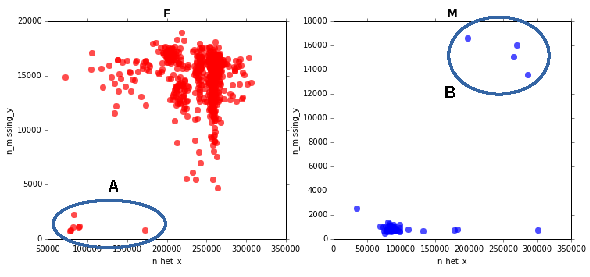
\includegraphics[width=\textwidth]{artwork/chapter3/sex.pdf}
\caption{Sex metadata concordance checks.
%
Each marker represents a sample.
%
The left panel (labelled F) shows samples from mosquitoes reported in metadata as female, the right panel (labelled M) shows samples reported as male.
%
$n\_het\_x$ = No. of heterozygous genotype calls on the $X$ chromosome.
%
$n\_missing\_y$ = No. of missing genotype calls on the $Y\_unplaced$ chromosome.
%
Groups labelled A and B are described in the text.
%
}
%
\label{fig:ch3-sex}
\end{figure}


%%
Both male and female mosquito specimens were contributed to Ag1000G phase 1 (Table~\ref{table:coverage}) and the morphologically-identified gender was included in the sample metadata contributed by the Ag1000G consortium partners who collected the specimens.
%
To confirm metadata records were correct, I compared the reported specimen gender with a gender call made directly from the sequencing data.
%
To call gender for each sample I computed the counts of homozygous, heterozygous and missing genotype calls separately for the X and Y chromosomes. 
%
Sex determination is similar in mosquitoes to humans in that females are homogametic XX and males are heterogametic XY.
%
Thus, in females we expect to observe heterozygous genotype calls on the X chromosome and missing genotype calls on the Y chromosome.
%
Conversely, in males we expect only homozygous genotype calls on the X chromosome and non-missing genotype calls on the Y chromosome.
%
Plotting these data it was evident that some samples had genotype counts not consistent with their reported sex (Fig.~\ref{fig:ch3-sex}).
%
This included six samples reported as female but with male genotype counts (Fig.~\ref{fig:ch3-sex} group A) and four samples reported as male but with female genotype counts (Fig.~\ref{fig:ch3-sex} group B).
%
I excluded these ten samples from further analyses.
%
There were also a further six samples with apparently androgynous genotype counts on sex chromosomes.
%
Cross-checking against the contamination analysis showed these apparently androgynous samples to have predicted contamination $>2\%$, explaining the unusual sex chromosome genotype counts.
%%


%%%%%%%%%%%%%%%%%%%%%%%%%%%%%%%%%%%%%%%%%%%%%%%%%%%%%%%%%%%%%%%%%%%%%%%%%%%%%%%
\subsubsection{Population outliers}


\begin{figure}[t!]
\centering
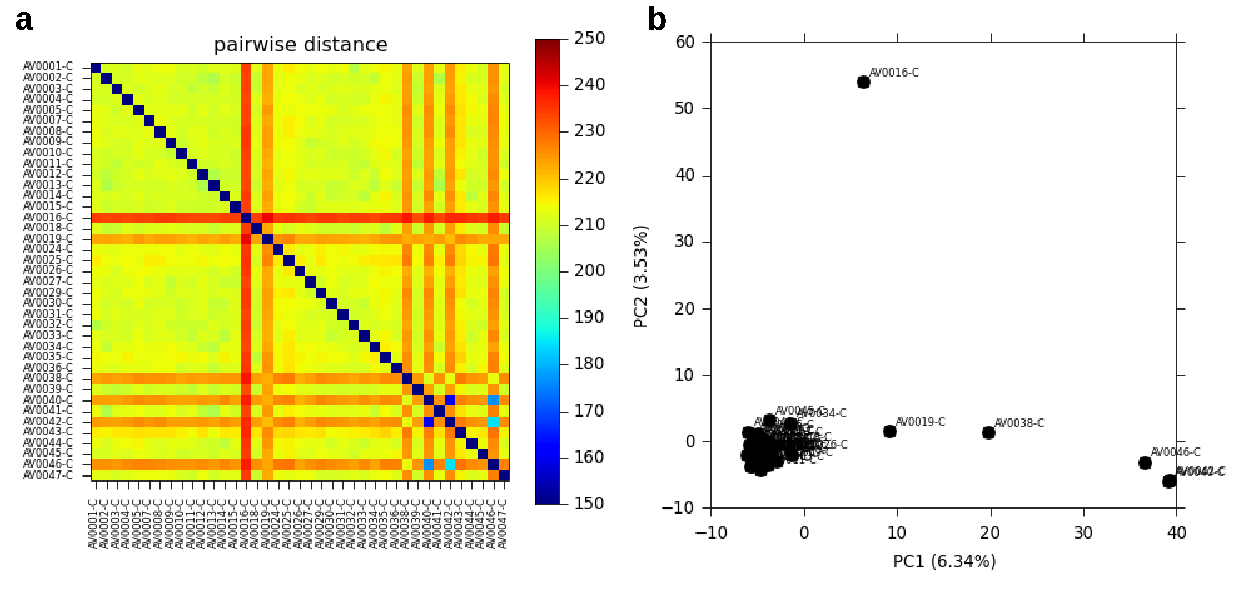
\includegraphics[width=\textwidth]{artwork/chapter3/popout.pdf}
\caption{Example of population outlier analysis for Guinea \textit{An. gambiae}.
%
Six samples are evident as outliers, having elevated genetic distance and appearing as outliers in PCA.
%
\textbf{a}, Pairwise genetic distance between samples, visualised as a heatmap.
%
\textbf{b}, PCA showing first and second principal components.
%
}
%
\label{fig:ch3-popout}
\end{figure}


%%
Mosquitoes in the phase 1 cohort represented 8 countries and two species. 
%
In Burkina Faso, both \agam\ and \acol\ were represented, whereas in all other countries only a single species was represented (either \agam\ or \textit{An. coluzzii}), except for Guinea-Bissau and Kenya where the species status was uncertain (Chapter 4).
%
In some countries, specimens had been collected from multiple sites, but in all cases the sites were within a relatively small geographical distance (Fig.~\ref{fig:ch3-map}).
%
Thus, in general we would expect to see little or no genetic structure among the specimens of any given species sampled from within a single country.
%
To confirm that the country of origin reported for each specimen in the sample metadata provided by Ag1000G consortium partners was consistent with the patterns of genetic population structure present in the data, I performed an outlier analysis using both pairwise genetic distance and principal components analysis (PCA)~\parencite{Patterson2006}).
%
In this analysis I used SNPs from Chromosome 3, then grouped samples by reported country and species, then performed both PCA and pairwise distance analyses on each group in turn (e.g., Fig.~\ref{fig:ch3-popout}).
%
If any samples were present in a group because of incorrect geographical or species metadata, they would be expected to appear as an outlying group of samples, with elevated genetic distance from other samples, and appearing as outliers in PCA.
%
In total, I identified and excluded 55 samples as population outliers.
%%


%%%%%%%%%%%%%%%%%%%%%%%%%%%%%%%%%%%%%%%%%%%%%%%%%%%%%%%%%%%%%%%%%%%%%%%%%%%%%%%
\subsubsection{Minimum depth of coverage}


\begin{figure}[t!]
\centering
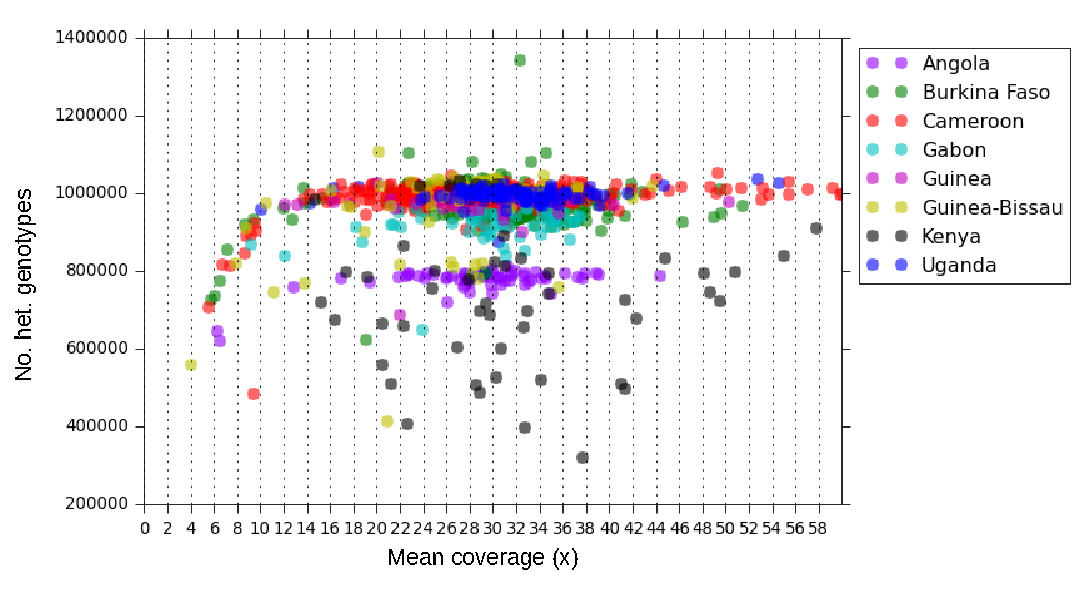
\includegraphics[width=\textwidth]{artwork/chapter3/coverage_hetz.pdf}
\caption{Coverage and heterozygosity.
%
Each marker represents a sample, coloured by country of collection.
%
No. het. genotypes = number of heterozygous genotype calls on autosomal chromosomes.
%
}
%
\label{fig:ch3-coverage_hetz}
\end{figure}


%%
In the analysis of sequence data quality described above I excluded samples with less than 80\% of the reference genome covered by at least one read, which is a conservative way to remove samples that are highly likely to have excessive levels of missingness in their genotype calls.
%
However, for accurate genotyping calling, particularly of heterozygous genotype calls, it is necessary to have sufficient depth of coverage.
%
Previous studies of SNP calling from whole genome sequencing data have found that coverage of $12\times$ is sufficient for calling heterozygous genotypes accurately~\parencite{Meynert2014}.
%
I examined the total number of heterozygous genotype calls on autosomal chromosomes among the Ag1000G phase 1 samples, plotted against the genome-wide average depth of coverage, for the remaining samples not previously excluded in other sample QC analyses (Fig.~\ref{fig:ch3-coverage_hetz}).
%
Although there are clear differences in the degree of heterozygosity in samples from different countries, which likely reflects differences in genetic diversity of the sampled populations, below $14\times$ there is a clear trend towards lower heterozygous genotype calls.
%
This could indicate an effect such as a bias in the underlying genotype calling, whereby heterozygous genotypes are undercalled at lower coverage.
%
To mitigate this I excluded samples with coverage $<14\times$ from the final dataset.
%%



%%%%%%%%%%%%%%%%%%%%%%%%%%%%%%%%%%%%%%%%%%%%%%%%%%%%%%%%%%%%%%%%%%%%%%%%%%%%%%%
\subsection{Variant quality control}\label{subsec:variant-quality-control}


%%
Variant calling algorithms such as GATK \textit{UnifiedGenotyper} are typically configured by default for high sensitivity, which means that the raw variant calls they emit contain a high rate of false positive variants.
%
Errors in variant calling can occur due to a variety of causes:
\begin{itemize}
%
\item \textbf{Sequencing errors.} With high depth of coverage, given the low error rate of Illumina sequencing, it is unlikely that sequencing errors will generate false SNP calls, because sequencing errors are generally random and unlikely to co-occur at the same genomic location in read alignments.
%
However, in some cases sequencing errors can be systematic, such as in the vicinity of mononucleotide repeats.
%
\item \textbf{Alignment errors.} Errors can occur in the alignment process, where reads originating from one genomic location are improperly aligned to a different genomic location.
%
Any differences between the sequences at the two genomic locations then appear as variants in the misaligned reads.
%
Alignment errors are particularly likely to occur in repetitive genome regions, where sequences at different locations are identical or share a high degree of homology.
%
Several types of repetitive DNA are common throughout eukaryotic genomes:
%
\begin{itemize}
%
\item \textbf{Low complexity regions}, e.g., sequences with a very high (A+T) content.
%
\item \textbf{Tandem repeats}, where some short sequence of nucleotides is repeated adjacently many times.
%
\item \textbf{Interspersed repeats}, where similar sequences are located at dispersed regions throughout the genome, commonly due to mobile genetic elements such as retrotransposons~\parencite{Tu2004,FernandezMedina2011}.
%
\end{itemize}
%
\item \textbf{Large structural variation.} Large copy number amplifications or deletions can cause errors when attempting to call smaller variants such as SNPs within the same genomic region or in close vicinity.
%
In particular, if a sample has a copy number amplification relative to the reference genome, sequence reads from both copies of the amplified region will be aligned to the same location in the reference genome.
%
If there is any sequence divergence between the different copies of the amplified region, this can appear as heterozygous SNPs within the sample.
%
\item \textbf{Sequence divergence.} If individuals contain sequence within their genomes with a higher degree of divergence from the reference genome, some or all reads may fail to be aligned at all at that location.
%
This results in a failure to observe some alleles, and a bias towards calling true heterozygous genotypes as homozygous, also known as allelic dropout.
%
\item \textbf{Reference genome assembly errors.} In any region where the reference genome has been incorrectly assembled, attempting to align sequences reads to that region may lead to spurious variant calls.
%
\end{itemize}
%
In this subsection I describe analyses performed to reduce the false discovery rate within a raw variant callset by designing and applying variant filters.
%%


%%%%%%%%%%%%%%%%%%%%%%%%%%%%%%%%%%%%%%%%%%%%%%%%%%%%%%%%%%%%%%%%%%%%%%%%%%%%%%%
\subsubsection{Genome accessibility}


%%
As a first step towards designing variant filters, I performed an analysis of genome accessibility, which determines which positions throughout the genome support unambiguous read alignments, and where there is minimal evidence for structural variation between samples. 
%
In this analysis I first computed detailed alignment statistics from read pileups for each sample at each position in the reference sequence, including the total depth of coverage, the fraction of reads aligned in a proper pair, the fraction of reads aligned ambiguously (mapping quality zero), and the root-mean-square mapping quality.
%
In order to accelerate this computation I developed the software package pysamstats\footnote{\url{https://github.com/alimanfoo/pysamstats}}.
%
I then aggregated these data across all samples, to obtain the following genome accessibility metrics at each genome position:
%
\begin{itemize}
%
\item \textbf{No Coverage.} The number of samples in which there were no reads aligned at the site (0-100\%).
%
\item \textbf{Low Coverage.} The percentage of samples in which depth of coverage was less than half the modal coverage for the whole genome (0-100\%).
%
\item \textbf{High Coverage.} The percentage of samples in which the depth of coverage was more than twice the modal coverage for the whole genome (0-100\%).
%
\item \textbf{Ambiguous Alignment.} The percentage of samples in which more than 10\% of aligned reads are aligned with mapping quality zero, indicating they could equally well have been aligned at another genomic location (0-100\%).
%
\item \textbf{Low Mapping Quality.} The percentage of samples in which the root-mean-square mapping quality was less than 30 (0-100\%).
%  
\item \textbf{Low Read Pairing.} The percentage of samples in which less than 90\% of reads were flagged as being aligned in a proper pair, meaning that the read and its mate pair were aligned in the correct orientation within a reasonable distance of each other (0-100\%).
\end{itemize}
%%


%%
I also obtained repeat annotations for the AgamP3 reference genome for VectorBase.
%
These comprise annotations from three algorithms: RepeatMasker, Tandem Repeat Finder (TRF) and DUST.
%
The DUST algorithm was originally a module within BLAST~\parencite{Altschul1990} and is designed to mask low complexity sequences only.
%
The RepeatMasker software~\parencite{Smit2013} is primarily designed for masking interspersed repeats matching a library of known repeat sequences (transposable elements etc.).
%
TRF~\parencite{Benson1999} specializes in locating tandem repeats.
%
These provided three additional genome accessibility metrics:
%
\begin{itemize}
%
\item \textbf{TRF.} The genome position is within a region annotated as a tandem repeat by the tandem repeat finder software (True/False).
%
\item \textbf{RepeatMasker.} The genome position is within a region annotated as a repeat by the RepeatMasker software (True/False).
%
\item \textbf{DUST.} The genome position is within a region marked as low complexity by the DUST software (True/False).
%
\end{itemize}
%%


\begin{figure}[t!]
\centering
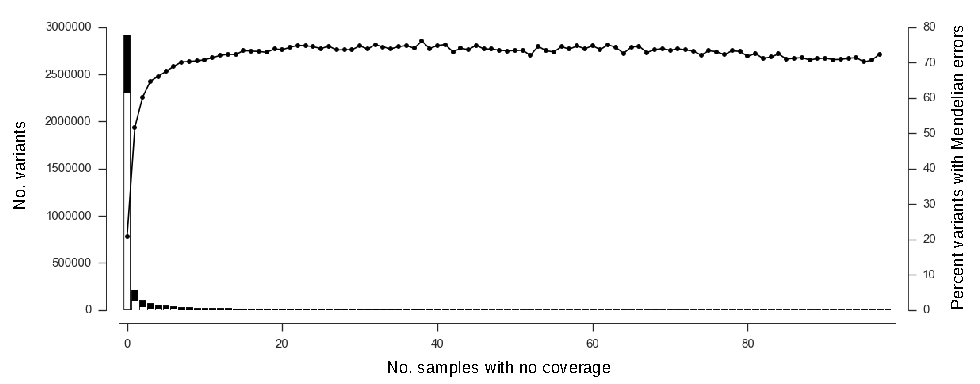
\includegraphics[width=\textwidth]{artwork/chapter3/me_nodp.pdf}
\caption{Example of using Mendelian error to calibrate thresholds for genome accessibility metrics.
%
Plot shows the Mendelian error (ME) rate for the No Coverage metric which measures the number of samples with no coverage at a given variant site.
%
Bars and left axis show the numbers of variants found for each value of the metric (black = variants with at least one ME; white = variants with no ME).
%
Line and right axis show the percentage of variants found with ME for each value of the metric.
%
}
%
\label{fig:ch3-me_nodp}
\end{figure}


%%
In previous population sequencing projects such as \textcite{1000G2015} the criteria used to determine which positions of the reference genome are considered accessible were decided theoretically, without any empirical validation.
%
The availability of colony crosses in the Ag1000G project afforded the opportunity to select and calibrate appropriate genome accessibility criteria using Mendelian error in the crosses as an indicator of poor accessibility.
%
The rationale here is that true variants will segregate within a cross according to Mendelian inheritance, whereas as false positive variants due to any of the above mentioned error modes would not in general be expected to segregate according to Mendelian inheritance, and thus be enriched for Mendelian errors.
%
A very small number of Mendelian errors are expected due to \textit{de novo} mutation, but the vast majority will be due to spurious variant calling, and hence Mendelian errors are a good indicator of poor quality variant calls~\parencite{Saunders2007,Laurie2010,Pilipenko2014}.
%
As a secondary means of empirically investigating genome accessibility, I also studied the ratio of transition to transversion substitutions (Ti/Tv).
%
Most organisms have mutation bias leading to an excess of transitions over transversions relative to that which would be expected if substitution mutations occurred randomly~\parencite{Guo2013}.
%
A low Ti/Tv ratio (approaching 0.5 expected if variants were called randomly) is an indicator of poor variant quality.
%
For each of the genome accessibility metrics listed above, I divided the range of possible values into bins, and then for each bin computed (1) the rate of Mendelian error as the fraction of variants in one or more crosses with genotypes not consistent with Mendelian segregation (ME); and (2) the Ti/Tv rate for biallelic SNPs.
%
I then plotted these results to identify bins within which ME was elevated and/or Ti/Tv was depressed (e.g., Fig.~\ref{fig:ch3-me_nodp}).
%%


%%
All the genome accessibility metrics displayed some structured association with Mendelian error and Ti/Tv, with higher metric values being associated with higher ME rates and lower Ti/Tv.
%
This was strongest for the No Coverage and Ambiguous Alignment metrics.
%
E.g., at positions where zero samples had No Coverage, the ME rate was 20\%, whereas at sites where three or more samples had No Coverage, the ME rate was 60\% or greater (Fig.~\ref{fig:ch3-me_nodp}).
%
Because some of these accessibility metrics would be expected to be correlated with each other to some extent, such as Ambiguous Alignment and Low Mapping Quality, I repeated the above analyses for each accessibility metric, but conditional on thresholds applied to all other metrics, to look for any marginal and thus unique contribution of a single metric.
%
In this analysis, all metrics remained informative, except for the Low Read Pairing metric.
%
I then decided the following criteria for genome positions to be classified as accessible:
%
\begin{itemize}
\item No Coverage <= 0.2\% (at most one sample with no coverage)
\item Ambiguous Alignment <= 0.2\% (at most one sample with 10\% MQ0 alignments)
\item High Coverage <= 2\% (at most 15 samples with high coverage)
\item Low Coverage <= 10\% (at most 76 samples with low coverage)
\item Low Mapping Quality <= 10\% (at most 76 samples with RMS MQ < 30)
\item DUST = False (position not annotated as a repeat by DUST)
\end{itemize}
%%


\begin{figure}[t!]
\centering
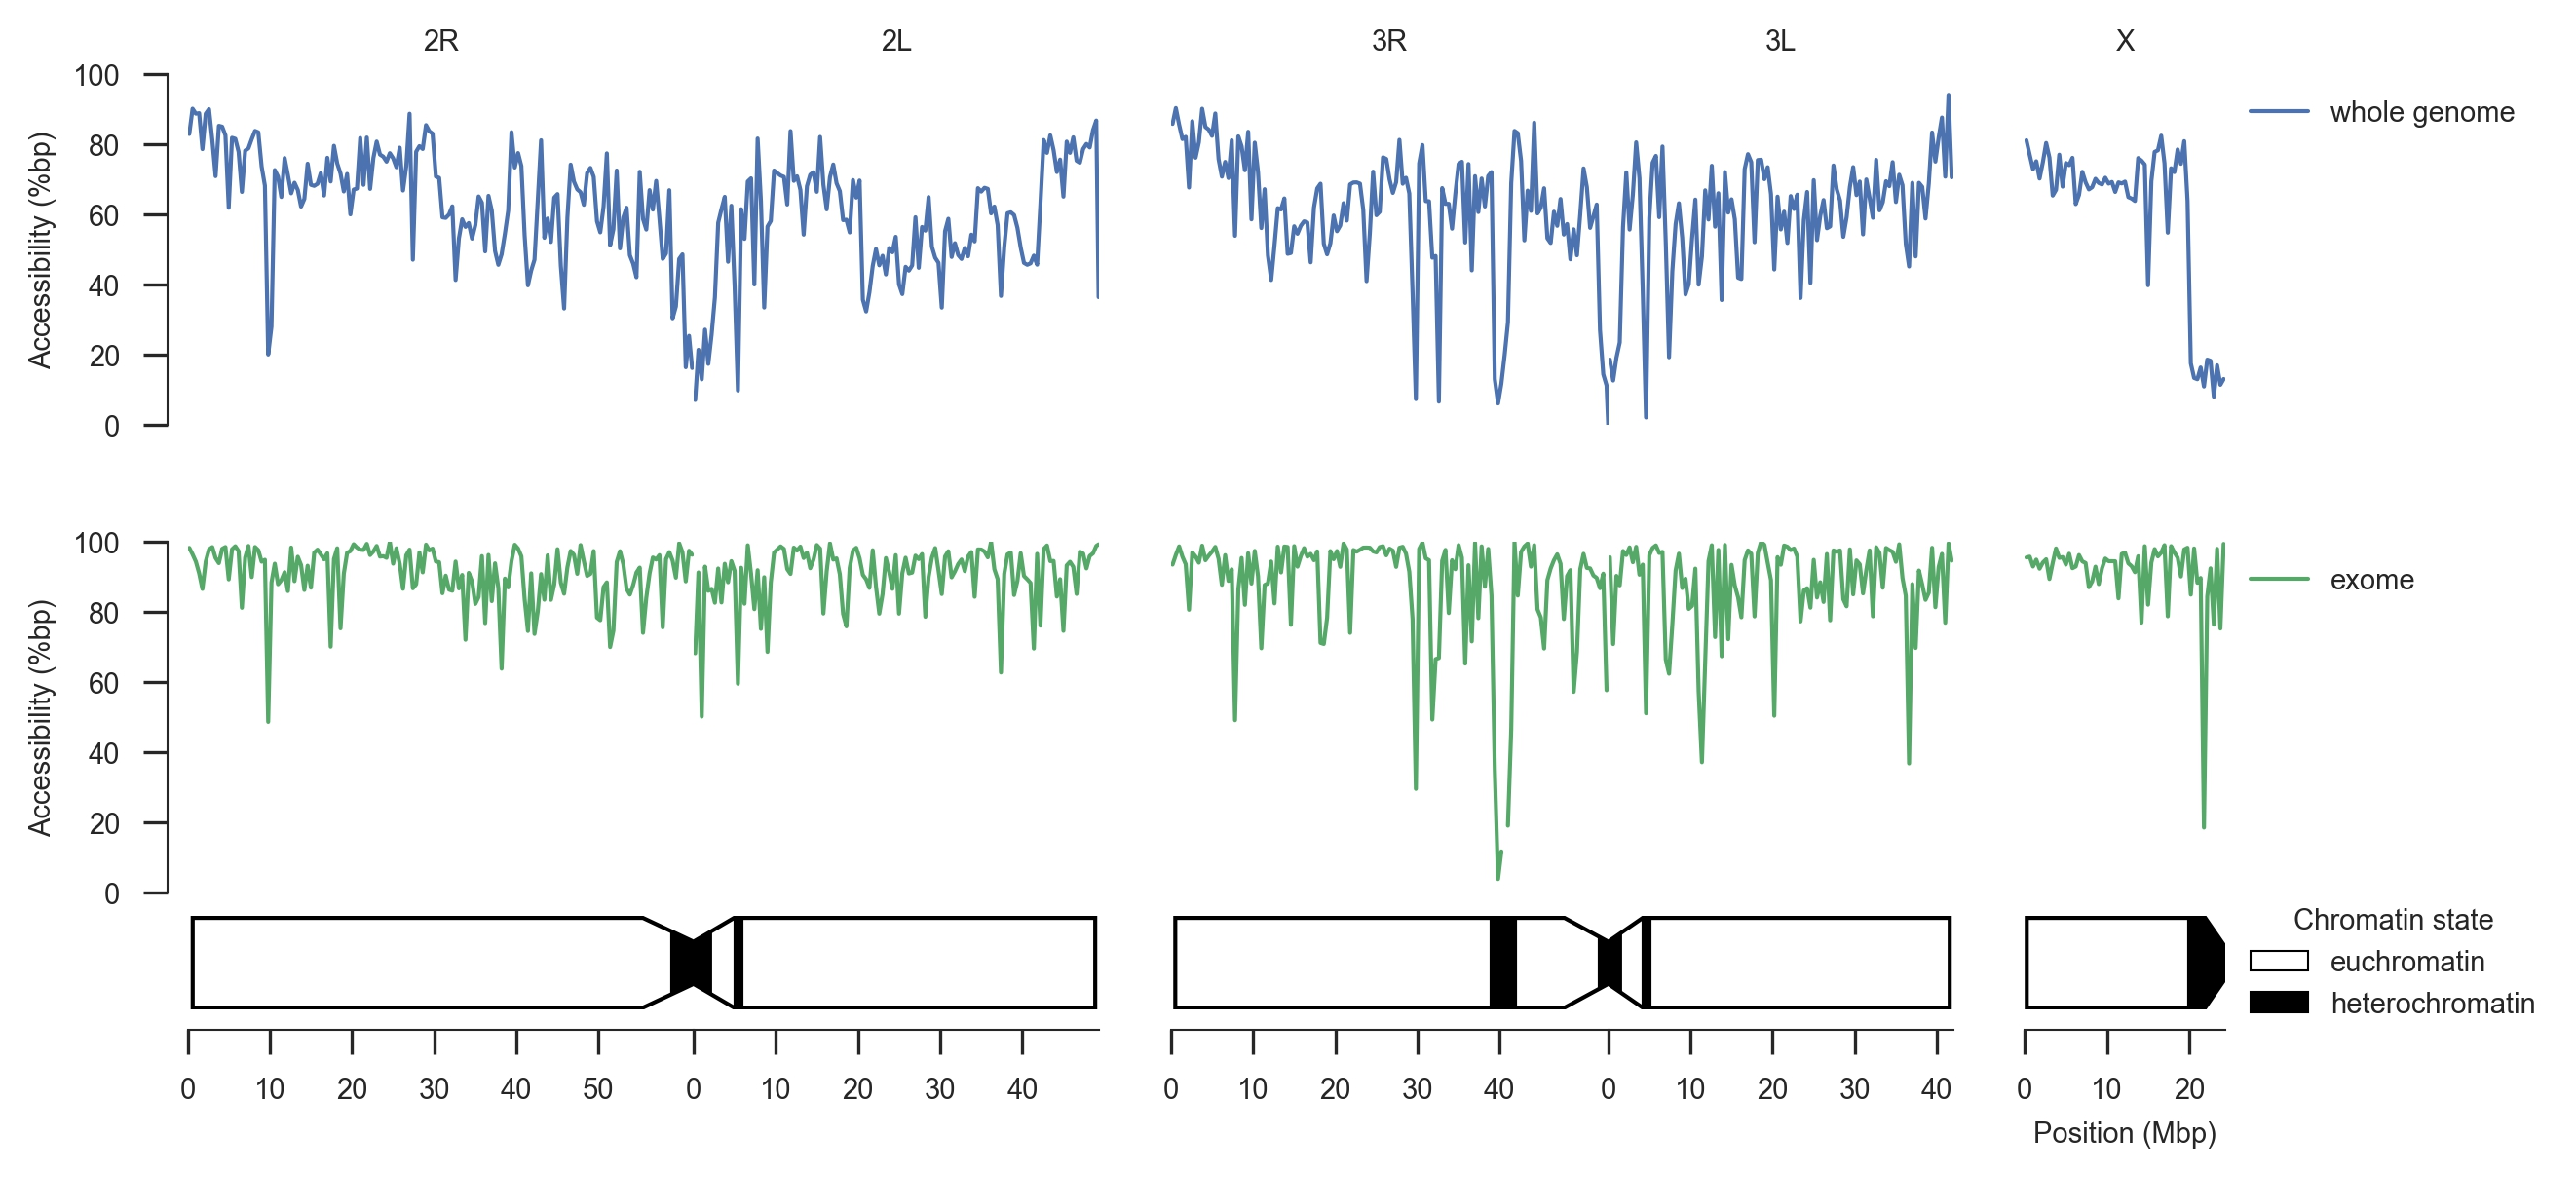
\includegraphics[width=\textwidth]{artwork/chapter3/accessibility.jpeg}
\caption{Results of genome accessibility analysis.
%
Upper plot (blue) shows the percentage of bases classified as accessible.
%
Lower plot (green) shows the percentage of bases within gene exons classified as accessible.
%
Schematic of chromosomes at the bottom shows predicted chromatin state from~\textcite{Sharakhova2010}.
%
}
%
\label{fig:ch3-accessibility}
\end{figure}


%%
After applying these criteria, 141 Mbp (61\% of the reference genome) was classified as accessible, including 91\% (18Mbp) of the exome and 60\% (123Mbp) of non-coding positions (Fig.~\ref{fig:ch3-accessibility}).
%
There were some clear associations between broad-scale patterns of accessibility and major features of genome architecture.
%
In particular, the pericentromeric regions of all three chromosomes, within regions predicted to be heterochromatic~\parencite{Sharakhova2010}, all displayed substantially lower accessibility.
%
This is likely due to a higher content of repetitive DNA sequence.
%
The region on chromosome arm 2L within the known polymorphic chromosomal inversion 2La~\parencite{Coluzzi2002}, which spans from 2L:20.5--42.2 Mb, also displayed lower accessibility.
%
This inversion is known to be segregating in many populations, and the inverted karyotype displays higher levels of divergence with respect to the standard karyotype represented in the reference genome sequence, thus this is likely an effect of divergence.
%%


%%%%%%%%%%%%%%%%%%%%%%%%%%%%%%%%%%%%%%%%%%%%%%%%%%%%%%%%%%%%%%%%%%%%%%%%%%%%%%%
\subsubsection{Variant filters}


%%
The raw variant callset produced by GATK \textit{UnifiedGenotyper} comprised a total of 95,335,499 SNPs distributed across the whole genome.
%
I designed a set of filters to annotate those SNPs likely to be false discoveries, and thus provide a means of excluding them from downstream analyses.
%
I first filtered SNPs using the genome accessibility criteria defined above.
%
I.e., a SNP was filtered if any of the accessibility criteria for the corresponding genome position were not met.
%
I then examined a set of variant metrics produced by \textit{UnifiedGenotyper} for each SNP, including the following metrics:
%
\begin{itemize}
%
\item \textbf{QD.} ``Quality by depth'', calculated as the evidence for an alternate allele at the site (QUAL, phred-scaled probability of no variant) divided by the total depth of coverage in samples where the alternate allele was observed.
%
\item \textbf{FS.} Fisher's exact test for strand-bias.
%
Phred-scaled probability of observing the given numbers of reads aligned to the forward and reverse strand if these were equally likely.
%
\item \textbf{ReadPosRankSum.} Rank sum test for relative positioning of reference and alternate alleles within reads.
%
Some sequencing errors tend to occur towards the ends of reads, and this metric quantifies the extent of any bias in read positioning between reference and alternate alleles.
%
\item \textbf{HRun.} The length of any adjacent homopolymer run.
%
Homopolymer runs are enriched for sequencing errors in Illumina sequencing data.
%
\end{itemize}


\begin{figure}[t!]
\centering
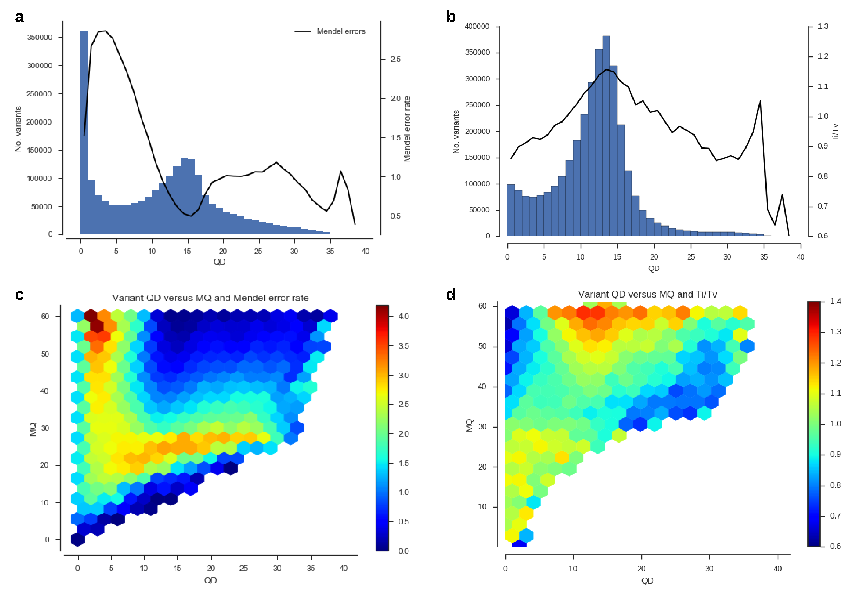
\includegraphics[width=1.1\textwidth,center]{artwork/chapter3/variant_filtering.pdf}
\caption{Examples of variant filter calibration analyses using Mendelian error and transition/transversion (Ti/Tv) ratio.
%
\textbf{a}, Analysis of QD and Mendelian error in a colony cross. Histogram shows the numbers of variants segregating in the cross on chromosome arm 3R, line shows percentage of those variants with at least one Mendelian error.
%
\textbf{b}, Analysis of QD and Ti/Tv. Histogram shows the number of variants segregating in the wild-caught samples, line shows the Ti/Tv ratio.
%
\textbf{c}, Joint analysis of QD, MQ and Mendelian error in a colony cross. Colour denotes the percentage of SNPs with at least one Mendelian error.
%
\textbf{d}, Joint analysis of QD, MQ and Ti/Tv. Colour denotes the Ti/Tv ratio for SNPs within each bin.
}
%
\label{fig:ch3-variant_filters}
\end{figure}


%%
Taking a similar approach to the genome accessibility analysis, I used Mendelian error in the crosses and Ti/Tv ratios to investigate which variant metrics appeared to be informative with respect to variant calling errors, and where filter thresholds should be set (e.g., Fig.~\ref{fig:ch3-variant_filters}).
%
Based on these analyses I filtered SNPs that failed any of the following criteria: QD $< 5$; FS $> 60$; ReadPosRankSum $< -8$; HRun $> 4$.
%
Of 95,335,499 SNPs reported in the raw callset, 52,525,957 passed all filters.
%
Prior to filtering, the rate of Mendelian error in genotype calls expected to be heterozygous (0/1) in the progeny of the crosses (where parental genotypes were 0/0 x 1/1 or vice versa) was between 13.0-21.7\% depending on the cross.
%
After filtering, this error rate was 0.3-0.9\%.
%%


%%%%%%%%%%%%%%%%%%%%%%%%%%%%%%%%%%%%%%%%%%%%%%%%%%%%%%%%%%%%%%%%%%%%%%%%%%%%%%%
%%%%%%%%%%%%%%%%%%%%%%%%%%%%%%%%%%%%%%%%%%%%%%%%%%%%%%%%%%%%%%%%%%%%%%%%%%%%%%%
\subsection{Production of an analysis-ready genome variation dataset}\label{subsec:production-of-an-analysis-ready-dataset}


%%
I produced an analysis-ready dataset in variant call format (VCF) for each chromosome arm by applying the sample and variant QC results described above as follows.
%
From all stages of sample QC a total of 123 samples were excluded, leaving 765 samples from wild-caught specimens passing all sample QC checks.
%
Taking the raw variant calls as input, I first removed all non-SNP variants, then removed genotype calls for individuals failing sample QC, then removed any SNPs that were no longer variant after excluding samples, using GATK \textit{SelectVariants}.
%
I then added INFO annotations with genome accessibility metrics, and added FILTER annotations recording the variant QC decisions, using bcftools \textit{annotate}.
%
Finally, I added INFO annotations with information about functional consequences of SNPs using SNPEFF version 4.1b~\parencite{Cingolani2012}.
%
After building VCF files, I also performed a conversion of these data to the HDF5 format, which is a general-purpose binary file format for scientific data that provides a significantly more performant way to load the variation data for downstream analysis.
%
I developed the software package vcfnp\footnote{\url{https://github.com/alimanfoo/vcfnp}} for performing this VCF to HDF5 format conversion.
%%


In order to support a broader range of population genetic analyses, the SNP genotypes in the 765 wild-caught individuals were also phased into haplotypes at the 41,476,870 biallelic sites.
%
In order to maximise the quality of the haplotypes, the phasing pipeline made use of both read-backed and statistical phasing methods~\parencite{Delaneau2013}.
%
Implementation and validation of the phasing pipeline was performed by Nick Harding from the MalariaGEN Resource Centre team, and is described in more detail in \textcite{Ag1000G2017}.
%
I supported this effort by developing an efficient algorithm for phasing the parents of the colony crosses using pedigree information, allowing the parents' haplotypes to be used as a gold standard for quantifying phasing error rates. 


%%
All the analysis-ready data files were uploaded to the Wellcome Sanger Institute public FTP site and are available at \url{ftp://ngs.sanger.ac.uk/production/ag1000g/phase1/}.
%
Sequence read alignments and analysis-ready variant calls were submitted to the European Nucleotide Archive (ENA; \url{http://www.ebi.ac.uk/ena}) under ENA study PRJEB18691.
%
I also collaborated with members of the MalariaGEN Web Application development team to design a web application to allow interactive exploration and browsing of these data, available at \url{http://www.malariagen.net/apps/ag1000g}.
%
Briefly, this web application provides the following features: queryable tables of variants and samples;
interactive plotting of variants and samples;
genome browser allowing visual exploration of tracks against their physical position within a chromosome arm, including genome accessibility metrics, variant quality metrics, various population genetic metrics, and visualisation of genotype calls within individual samples.
%%


%%%%%%%%%%%%%%%%%%%%%%%%%%%%%%%%%%%%%%%%%%%%%%%%%%%%%%%%%%%%%%%%%%%%%%%%%%%%%%%
%%%%%%%%%%%%%%%%%%%%%%%%%%%%%%%%%%%%%%%%%%%%%%%%%%%%%%%%%%%%%%%%%%%%%%%%%%%%%%%
\subsection{Validation with Sanger sequencing}\label{subsec:validation-with-sanger-sequencing}


%%
To provide an independent estimate for the SNP false discovery rate (FDR) and sensitivity, Sanger sequencing was performed of five loci in 58 individual mosquitoes that were also analysed using whole genome sequencing.
%
The primers were provided by the Liverpool School of Tropical Medicine, and the Sanger sequencing was performed by the MalariaGEN Resource Center team at the Wellcome Centre for Human Genetics.
%
The individuals used in the validation analysis included representatives of all sampling locations except Kenya.
%
Loci were sequenced using the following sets of forward and reverse primer pairs: 
%
\begin{itemize}
\item 3R:6,906,804-6,908,373 \\ ACTGATCGAGGTAGGGCATC/CGCATCGAGTCCAATCTTTT
\item 3L:22,022,788-22,024,835 \\ ACCCTCGTCTTTCACCACAC/CATCCACCGGAGTACTTGCT
\item 3L:39,820,960-39,822,628 \\ GGTAGCAGTCGCCAGTTTTT/CTTGAGCGCCACCTTAAGTC
\item 2L:46,845,944-46,847,857 \\ GGAGTTTTACGTGGCCGTTA/CTTCAAAGTGCGGATCCATT 
\item 2R:28,491,415-28,493,141 \\ TTCAAGTAGTTGCCCGCTTT/AATCGAGCTATTGCGGAGAA
\end{itemize}


For each primer set, I aligned forward and reverse traces and called SNPs and genotypes using NovoSNP version 3.0.1~\parencite{Weckx2005}.
%
I analysed only individuals which had high quality traces for both forward and reverse reads spanning at least 90\% of the distance between primers.
%
I also excluded individuals where there was evidence for heterozygous indel variation.
%
I defined true positives, false positives and false negatives by comparing variant calls derived from the Illumina and Sanger data for the individuals sequenced with both technologies.
%
I defined a false positive as a SNP called from Illumina sequence data for which there was no evidence on either forward or reverse Sanger traces in any individuals.
%
I defined a false negative as a SNP for which there was evidence in at least one individual on both forward and reverse Sanger traces but which was not called from Illumina sequence data.
%
A SNP present in the Illumina calls for these individuals and in the Sanger calls was defined as a true positive.
%
FDR was computed as the number of true positives divided by the number of true positives plus false positives.
%
In total, there were 261 true positives and 1 false positive, an FDR of 1/262 = 0.4\%.
%
The false positive SNP was observed in only a single individual, as a heterozygous genotype.
%
Sensitivity was computed as the number of true positives divided by the number of true positives plus false negatives.
%
There were 15 false negatives at genome positions classified as accessible, a sensitivity of 261/276 = 94.6\%.
%
Sensitivity across the five loci ranged from 88.5\%-100\%.
%
I also compared genotype calls, finding that 984/1000 (98.4\%) of heterozygous genotype calls and 6881/6884 (99.96\%) of homozygous genotype calls were concordant between Sanger and Illumina data.
%%


%%%%%%%%%%%%%%%%%%%%%%%%%%%%%%%%%%%%%%%%%%%%%%%%%%%%%%%%%%%%%%%%%%%%%%%%%%%%%%%
%%%%%%%%%%%%%%%%%%%%%%%%%%%%%%%%%%%%%%%%%%%%%%%%%%%%%%%%%%%%%%%%%%%%%%%%%%%%%%%
%%%%%%%%%%%%%%%%%%%%%%%%%%%%%%%%%%%%%%%%%%%%%%%%%%%%%%%%%%%%%%%%%%%%%%%%%%%%%%%
\section{Results}\label{sec:ch3-results}


%%%%%%%%%%%%%%%%%%%%%%%%%%%%%%%%%%%%%%%%%%%%%%%%%%%%%%%%%%%%%%%%%%%%%%%%%%%%%%%
%%%%%%%%%%%%%%%%%%%%%%%%%%%%%%%%%%%%%%%%%%%%%%%%%%%%%%%%%%%%%%%%%%%%%%%%%%%%%%%
\subsection{Nucleotide variation}\label{subsec:nucleotide-variation}


\begin{figure}[t!]
\centering
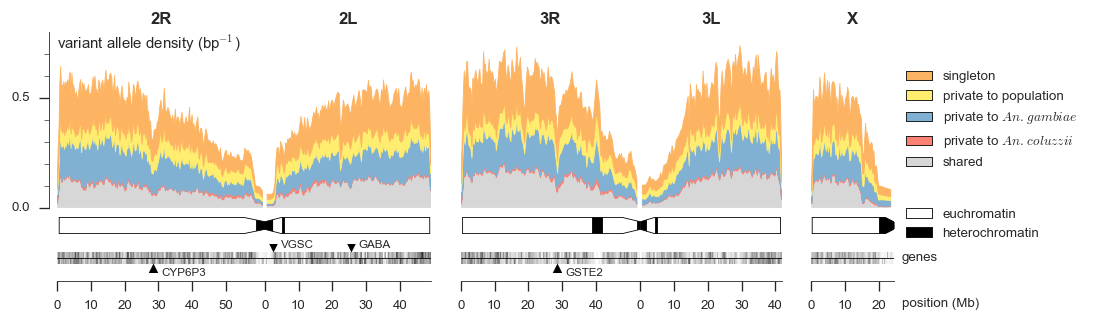
\includegraphics[width=1.1\textwidth,center]{artwork/chapter3/variant_density.png}
\caption{Density of variant alleles discovered across the genome.
%
Main plot shows the density of variant alleles per accessible base, computed in 200 kb moving windows.
%
Chromosome schematic below shows chromatin state predictions from \textcite{Sharakhova2010}.
%
\textit{Cyp6p3}, \textit{Vgsc}, \textit{Gaba} and \textit{Gste2} are genes known to be involved in insecticide resistance.
}
%
\label{fig:ch3-variant_density}
\end{figure}


52,525,957 SNPs were discovered in the Ag1000G phase 1 dataset passing all quality filters.
%
Of these, 41,476,870 (79\%) were biallelic and 11,049,087 (21\%) were multiallelic (more than one variant allele), giving a total of 64,481,991 variant alleles.
%
21,783,339 variant alleles were singletons (only observed as a heterozygous genotype in a single individual), 31,228,996 were observed only in a single country and species (private to a population), 17,144,828 were found in multiple countries but observed only in \textit{An. gambiae}, 1,252,245 were found in multiple countries but only in \textit{An. coluzzii}, and 14,688,252 were shared between the two species.


On average one variant allele was discovered every 2.2 bases of the accessible genome,
but variant alleles were not evenly distributed throughout the genome (Fig.~\ref{fig:ch3-variant_density}).
%
Variant allele density was lower towards the centromeres on all chromosome arms, and especially low within regions of pericentromeric heterochromatin where recombination is reduced~\parencite{Pombi2006,Zheng1997}.
%
Diversity is also lower near centromeres in \textit{D. melanogaster}~\parencite{Langley2012} and correlated with recombination rate across a variety of species due to selection at linked sites~\parencite{Charlesworth2012a,Elyashiv2016,
CorbettDetig2015,Burri2015,Chan2012,Spencer2006}.
%
Chromatin state was not always associated with lower variant density, however, as the region of intercalary heterochromatin on chromosome arm 3R had noticeably elevated variant density.
%
Drops in variant allele density, and particularly the density of singleton alleles, were visible at genome regions containing the insecticide resistance genes \textit{Cyp6p3} and \textit{Gste2}, suggesting the presence of selective sweeps in those genome regions, investigated further in Chapter 5.


Individual samples carried between 1.6 and 2.7 million variant alleles (Fig.~\ref{fig:ch3-sample_variant_count}).
%
There was no systematic difference between the two species, \agam\ and \textit{An. coluzzii}, in terms of the number of variant alleles discovered in each sample, indicating that the AgamP3 reference genome is not biased towards one species or the other.
%
However, there was a clear difference in the level of variation between the two species within the centromeric region of the X chromosome, where \agam\ populations had higher levels of variation than \acol, and thus the reference genome within that region is more representative of \acol\ (Fig.~\ref{fig:ch3-sample_variant_density}).
%
The 2La inversion also created a notable difference between individuals both within and between populations, consistent with polymorphism and substantial sequence divergence between the two karyotypes.
%%


%%%%%%%%%%%%%%%%%%%%%%%%%%%%%%%%%%%%%%%%%%%%%%%%%%%%%%%%%%%%%%%%%%%%%%%%%%%%%%%
%%%%%%%%%%%%%%%%%%%%%%%%%%%%%%%%%%%%%%%%%%%%%%%%%%%%%%%%%%%%%%%%%%%%%%%%%%%%%%%
\subsection{Gene architecture and genetic diversity}\label{subsec:gene-architecture-and-genetic-diversity}


%
Gene architecture is expected to exert a strong influence on the genomic landscape of nucleotide variation, because different components of protein-coding sequences are under different types and degrees of selective pressure.
%
For example, in general, exons of protein-coding genes will be under purifying selection, because the protein is under some functional constraint~\parencite{Ohta1996}.
%
Thus, genetic diversity within exons is expected to be lower than within introns or intergenic sequence.
%
However, the level of constraint will depend on whether nucleotides occur in the first, second or third codon position, because third codon positions have some degeneracy and nucleotide substitutions are less likely to cause an amino acid substitution than at the first or second codon position.
%
Although these phenomena are common to all eukaryotic genomes, there will be differences between species due to differences in their biology, genome size, mutation rate, recombination rate and effective population size.
%
The Ag1000G data resource provides an opportunity to investigate some of these features of genome biology in the context of a eukaryotic species with large effective population sizes.


\begin{figure}[t!]
\centering
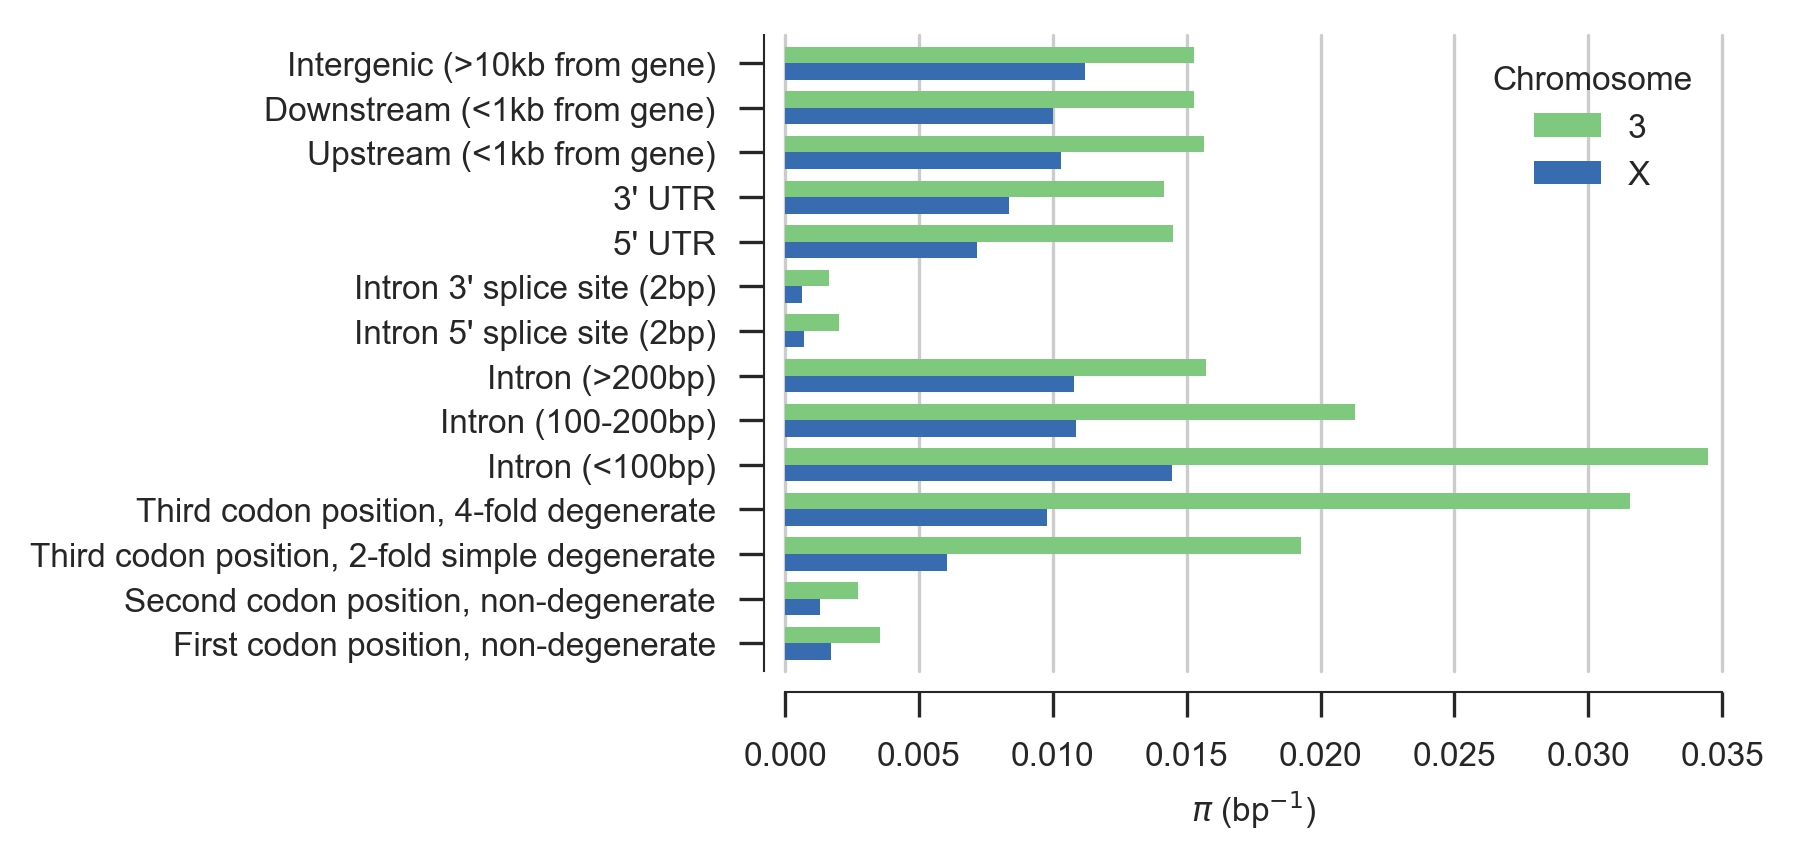
\includegraphics[width=1.1\textwidth,center]{artwork/chapter3/feature_pi.jpeg}
\caption{Nucleotide diversity ($\pi$) in relation to gene architecture.
}
%
\label{fig:ch3-feature_pi}
\end{figure}



%
Of the 52,525,957 SNPs discovered, 4,404,390 (8.4\%) occurred within a gene coding region (Table~\ref{table:snpeff}).
%
Of the SNPs within gene coding regions, 1,809,532 (41.1\%) were non-synonymous (missense) SNPs that altered the amino acid sequence of the gene, and the remaining 2,594,858 (58.9\%) were synonymous.
%
To further investigate the impact of gene architecture on levels of nucleotide variation, I computed nucleotide diversity ($\pi$) in the phase 1 cohort within different types of coding and non-coding sites (Fig.~\ref{fig:ch3-feature_pi}).
%
I computed diversity separately within the X chromosome and the autosomal Chromosome 3, because the X chromosome is hemizygous in males and thus has a lower effective population size as well as experiencing less frequent recombination than the autosomes, both of which may affect genetic diversity.
%
The lowest diversity was found within intronic splice sites, consistent with a high degree of purifying selection, because any change in gene splicing is likely to have major functional consequences.
%
The reduction of diversity at splice sites was strongest within the first 2 bp of the intronic sequence, but also extended up to 9 bp into the intron at the 5' end, although not at the 3' end (Fig.~\ref{fig:ch3-splicing_pi}).
%
Diversity was also low within exons at non-degenerate first and second codon positions, where any nucleotide substitution will cause an amino acid substitution, also consistent with strong purifying selection.
%
In contrast, diversity was much higher at fourfold degenerate coding sites, reaching 3.2\% on Chromosome 3, consistent with a lack of purifying selection.
%
The only sequence class where diversity was higher was within short ($<$100 bp) introns, where $\pi$ on Chromosome 3 was approaching 3.5\%.
%%


%%
Two other results of this analysis are interesting.
%
Firstly, on Chromosome 3 diversity was more than twice as high in short (<100 bp) introns than long (>200 bp) introns.
%
This suggests that longer introns are in general subject to greater functional constraint, for example, due to the presence of regulatory sequences.
%
Shorter introns might be too small to contain regulatory sequences, or might be younger and thus have had less time to evolve a regulatory function.
%
A similar pattern is seen in other insects and arthropods~\parencite{Singh2013,Martin2016,Lynch2016}, and is consistent with evidence in
\textit{Drosophila} that longer non-coding sequences are more likely to contain functional elements~\parencite{Casillas2007}.
%
Secondly, diversity in intergenic regions $>$10 kb distant from a gene was 1.5\%, similar to that in longer introns, and much lower than short introns or degenerate coding positions.
%
Diversity in intergenic regions was similar regardless of distance to a gene, suggesting that lower diversity is not due to genetic linkage and linked purifying selection, but reflects some substantial selective constraint on intergenic sequence.
%%


%%
There were also notable differences between the autosomal Chromosome 3 and the X chromosome in these patterns of diversity in relation to gene architecture.
%
Diversity was generally lower on the X chromosome across all site classes, as expected due to the fact that males carry only a single X chromosome and thus the effective population size is lower for the X chromosome than for the autosomes.
%
However, the ratio of diversity between sex chromosomes and autosomes (X/A ratio) differed between site classes (Fig.~\ref{fig:ch3-feature_pi_ratios}).
%
The X/A ratio was highest within intergenic regions $>$10 kb from a gene, with values between 0.63-0.76, close to the theoretical expectation of 0.75 due to reduced effective population size.
%
In contrast, the X/A ratio was lowest (0.27-0.32) at degenerate coding positions.
%
This suggests that genetic linkage and purifying selection at linked sites is a substantially stronger force reducing diversity on the X chromosome than the autosomes, because the X/A ratio is highest at sites furthest from genes.
%
This is consistent with the fact that meiotic recombination occurs only in females and is less frequent on the X chromosome than autosomes where recombination occurs in both sexes.
%
The X/A ratio can also be influenced by demographic factors, including population size fluctuations and sex biases in reproductive success and migration~\parencite{CorbettDetig2015,Webster2016,Pool2007,Charlesworth2012b}, and these may also be playing a role, although the X/A ratios were relatively stable across the different species and populations sampled in Ag1000G phase 1.
%



%%%%%%%%%%%%%%%%%%%%%%%%%%%%%%%%%%%%%%%%%%%%%%%%%%%%%%%%%%%%%%%%%%%%%%%%%%%%%%%
%%%%%%%%%%%%%%%%%%%%%%%%%%%%%%%%%%%%%%%%%%%%%%%%%%%%%%%%%%%%%%%%%%%%%%%%%%%%%%%
%%%%%%%%%%%%%%%%%%%%%%%%%%%%%%%%%%%%%%%%%%%%%%%%%%%%%%%%%%%%%%%%%%%%%%%%%%%%%%%
\section{Conclusions}\label{sec:ch3-conclusions}


In this chapter I have described the discovery and genotyping of more than 50 million single nucleotide polymorphisms from deep whole genome sequencing of individual mosquitoes from natural populations of \agam\ and \textit{An. coluzzii}.
%
This is a unique data resource, providing opportunities to study both fundamental genome biology and the evolution and demography of natural malaria vector populations.
%
I have shown that this is a highly robust data resource, with low rates of false discovery and highly accurate genotype calls.
%
I have also used this resource to show that nucleotide diversity is extremely high within these mosquito species, confirming that they are among the most genetically diverse organisms studied to date~\parencite{Leffler2012}.
%
In the next chapter I will use these data to investigate genetic structure among the populations sampled, and to quantify, characterise and compare genetic diversity within these populations in more detail.
%%


%%%%%%%%%%%%%%%%%%%%%%%%%%%%%%%%%%%%%%%%%%%%%%%%%%%%%%%%%%%%%%%%%%%%%%%%%%%%%%%
%%%%%%%%%%%%%%%%%%%%%%%%%%%%%%%%%%%%%%%%%%%%%%%%%%%%%%%%%%%%%%%%%%%%%%%%%%%%%%%
%%%%%%%%%%%%%%%%%%%%%%%%%%%%%%%%%%%%%%%%%%%%%%%%%%%%%%%%%%%%%%%%%%%%%%%%%%%%%%%
\section{Acknowledgments}\label{sec:ch3-acknowledgments}


I would like to thank the members of the \textit{Anopheles gambiae} 1000 Genomes Consortium, the MalariaGEN Resource Centre team, and the staff at the Wellcome Sanger Institute sample logistics, sequencing and informatics facilities, for their contributions towards the production of the Ag1000G phase 1 data resource.


\clearpage
%%%%%%%%%%%%%%%%%%%%%%%%%%%%%%%%%%%%%%%%%%%%%%%%%%%%%%%%%%%%%%%%%%%%%%%%%%%%%%%
%%%%%%%%%%%%%%%%%%%%%%%%%%%%%%%%%%%%%%%%%%%%%%%%%%%%%%%%%%%%%%%%%%%%%%%%%%%%%%%
%%%%%%%%%%%%%%%%%%%%%%%%%%%%%%%%%%%%%%%%%%%%%%%%%%%%%%%%%%%%%%%%%%%%%%%%%%%%%%%
\section{Supplemental figures}\label{sec:ch3-supplemental-figures}


\begin{figure}[h]
\centering
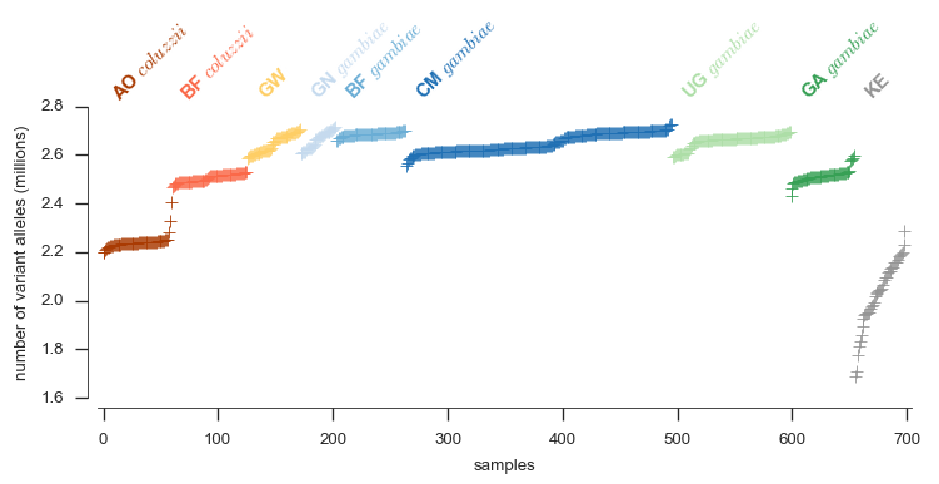
\includegraphics[width=1\textwidth,center]{artwork/chapter3/sample_variant_count.pdf}
\caption{Number of variant alleles by sample.
%
Each marker represents an individual sample, coloured by country and species.
%
Number of variant alleles is computed over the whole genome.
}
%
\label{fig:ch3-sample_variant_count}
\end{figure}


\clearpage
\begin{figure}[h]
\centering
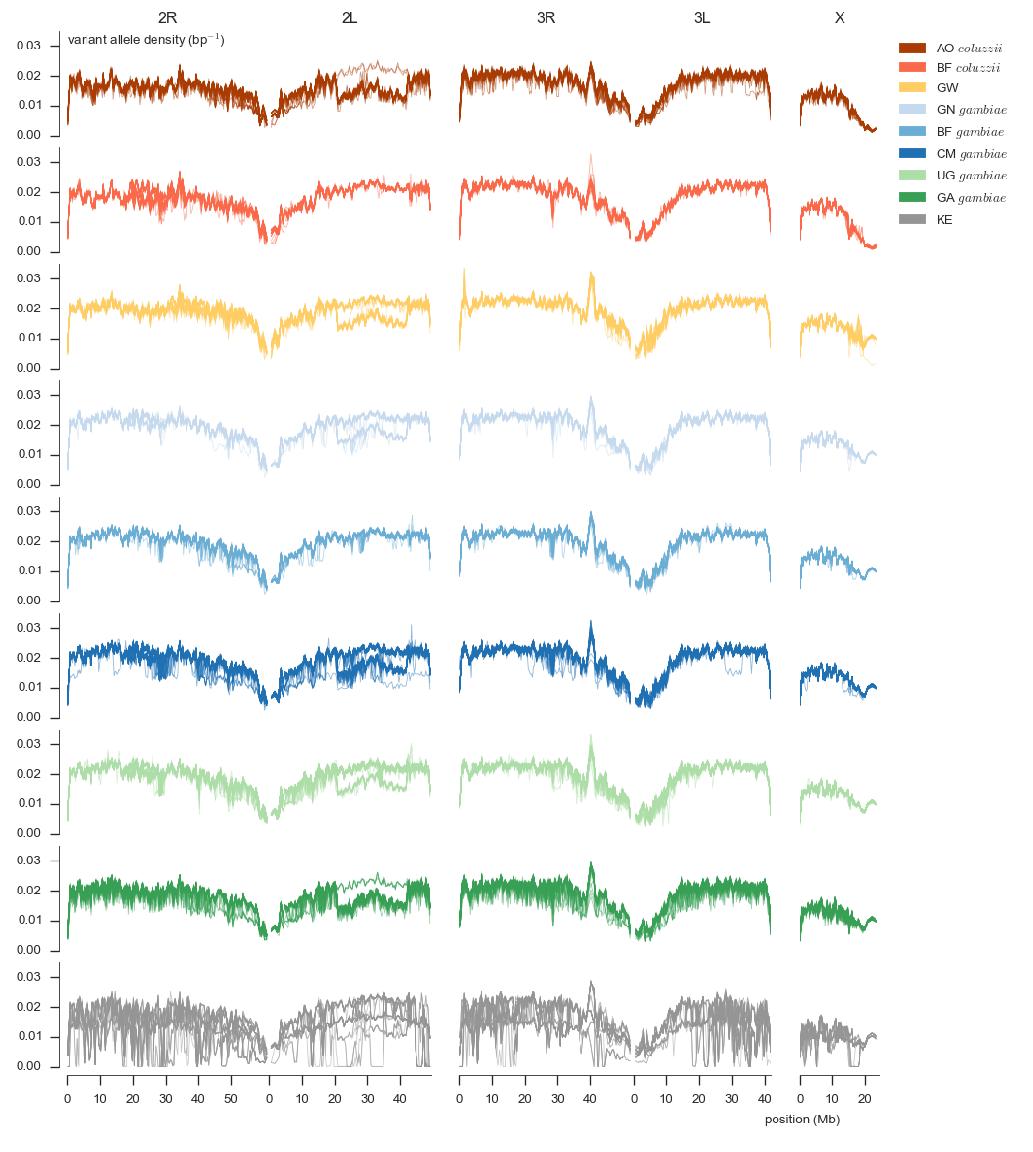
\includegraphics[width=1.1\textwidth,center]{artwork/chapter3/sample_variant_density.pdf}
\caption{Variant allele density by sample.
%
Each individual line plots variant allele density (number of variant alleles per accessible base) for a single sample in 200 kb windows across the genome.
%
Individuals are grouped by country and species to facilitate comparison within and between populations.
}
%
\label{fig:ch3-sample_variant_density}
\end{figure}


\clearpage
\begin{figure}[h]
\centering
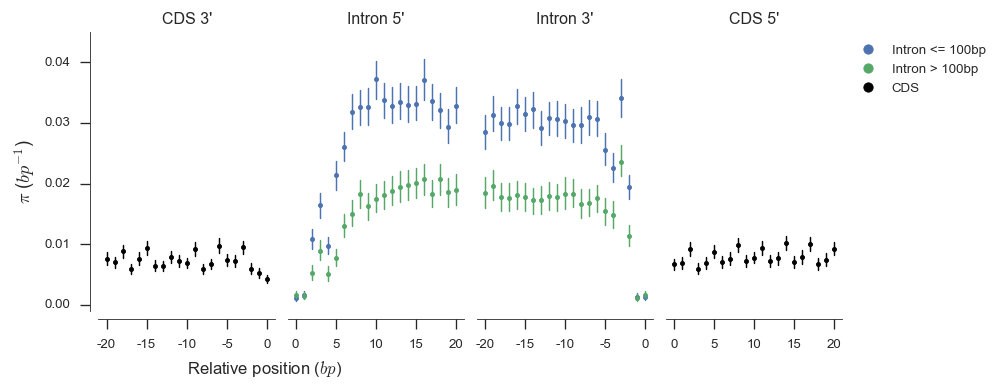
\includegraphics[width=1.1\textwidth,center]{artwork/chapter3/splicing_pi.png}
\caption{Nucleotide diversity ($\pi$) in relation to intron/exon boundaries.
%
Plots show diversity averaged across all genes on chromosome arm 3R, error bars show results from bootstrapping over sites.
}
%
\label{fig:ch3-splicing_pi}
\end{figure}


\clearpage
\begin{figure}[h]
\centering
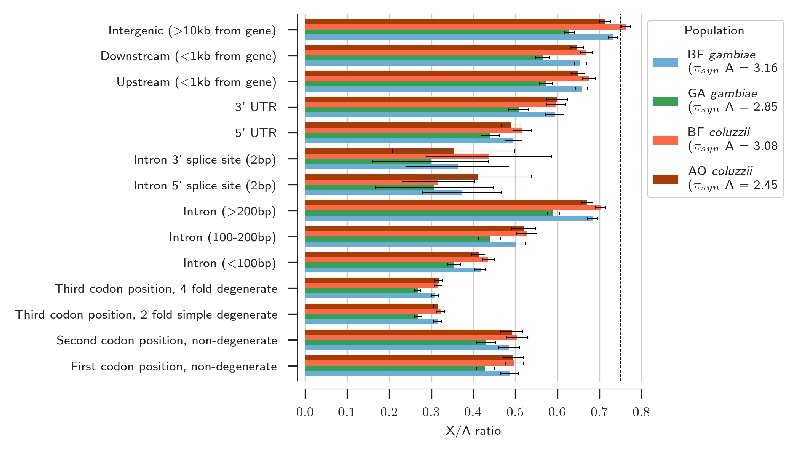
\includegraphics[width=1.1\textwidth,center]{artwork/chapter3/feature_pi_ratios.pdf}
\caption{Ratios of nucleotide diversity between the sex chromosome (X) and the autosomes (represented by Chromosome 3).
%
Error bars computed by bootstrapping over sites.
%
The theoretical expectation for a diploid species with one sex hemizygous for the X chromosome is 0.75 (shown as dashed line) due to differences in effective population sizes.
}
%
\label{fig:ch3-feature_pi_ratios}
\end{figure}


\clearpage
%%%%%%%%%%%%%%%%%%%%%%%%%%%%%%%%%%%%%%%%%%%%%%%%%%%%%%%%%%%%%%%%%%%%%%%%%%%%%%%
%%%%%%%%%%%%%%%%%%%%%%%%%%%%%%%%%%%%%%%%%%%%%%%%%%%%%%%%%%%%%%%%%%%%%%%%%%%%%%%
%%%%%%%%%%%%%%%%%%%%%%%%%%%%%%%%%%%%%%%%%%%%%%%%%%%%%%%%%%%%%%%%%%%%%%%%%%%%%%%
\section{Supplemental tables}\label{sec:ch3-supplemental-tables}


\begin{table}[h]
\begin{center}
\begin{threeparttable}

\caption{Number of SNPs discovered, grouped by sequence ontology annotation class as determined by SNPEFF~\parencite{Cingolani2012}.}

\label{table:snpeff}

\begin{tabular}{lr}
 \hline
 \textbf{Annotation} & \textbf{No. SNPs} \\
 \hline
intergenic\_region & 21,932,312 \\
intron\_variant & 11,040,938 \\
upstream\_gene\_variant & 8,960,291 \\
downstream\_gene\_variant & 5,012,563 \\
synonymous\_variant & 2,594,858 \\
missense\_variant & 1,809,532 \\
3\_prime\_UTR\_variant & 480,546 \\
5\_prime\_UTR\_variant & 325,007 \\
intragenic\_variant & 280,084 \\
splice\_region\_variant & 186,102 \\
5\_prime\_UTR\_premature\_start\_codon\_gain\_variant & 60,784 \\
stop\_gained & 15,744 \\
splice\_donor\_variant & 3,946 \\
splice\_acceptor\_variant & 3,117 \\
stop\_retained\_variant & 2,472 \\
stop\_lost & 1,546 \\
start\_lost & 1,444 \\
initiator\_codon\_variant & 257 \\
non\_canonical\_start\_codon & 10 \\
 \hline
\end{tabular}

\end{threeparttable}
\end{center}
\end{table}


\printbibliography[
heading=subbibintoc,
title={References}
]


\end{refsection}
